\documentclass[12pt,letterpaper]{article}

\usepackage[spanish]{babel}
\usepackage{graphicx}
\usepackage{float}
\usepackage{enumerate}

\author{Base de datos}
\title{Análisis de ingeniería inversa sobre un sistema \textit{legacy}}
\date{\today}

\begin{document}

\maketitle
\tableofcontents
\newpage

\section{Introducción}

\section{Descripción del problema}

\section{Análisis}

\section{Diagramas y resultados}

\subsection{Diagrama Entidad-Relación}

\begin{figure}[H]
    \centering
    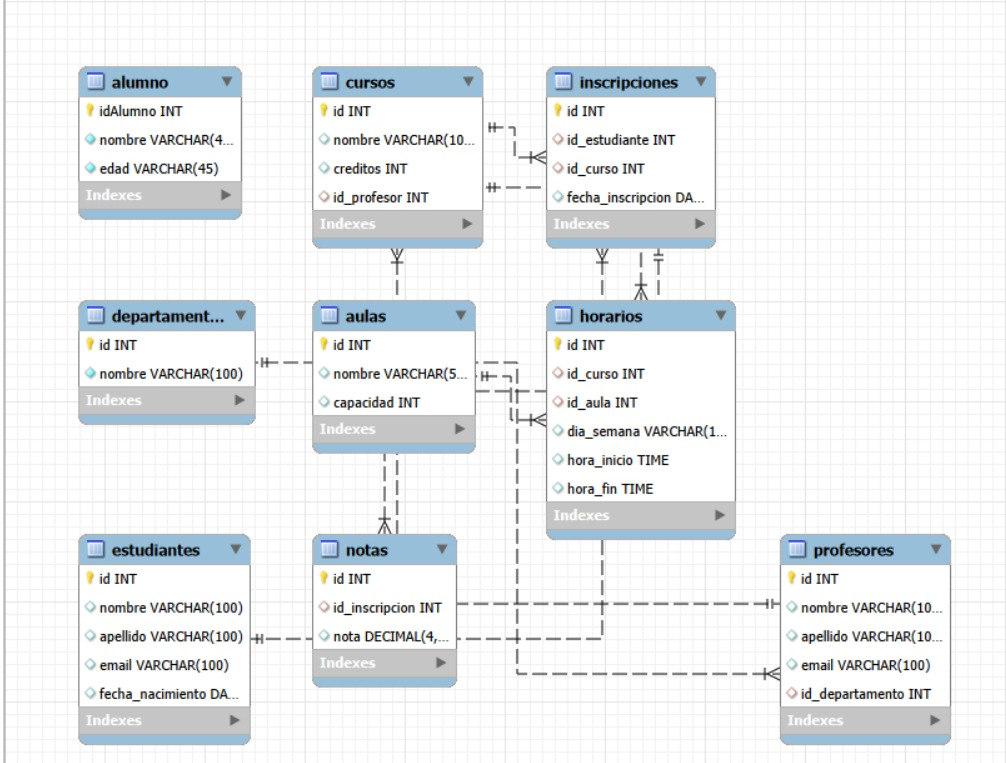
\includegraphics[width=0.8\textwidth]{imgs/diagrams.jpeg}
    \caption{Diagrama entidad-relación del sistema de escuela}
\end{figure}

\subsection{Resultados de las consultas}

\begin{enumerate}
\item ¿Cuáles son los estudiantes inscritos en el curso Álgebra?
\item ¿Qué cursos imparte el profesor Pedro Martínez?
\item ¿Cuántos estudiantes están inscritos en cada curso?
\item ¿Cuál es el promedio de notas por curso?
\item Lista de estudiantes con notas mayores a 8.0
\item ¿Qué cursos tienen más de una inscripción?
\item ¿Qué profesores pertenecen al departamento de Ingeniería?
\item ¿Cuáles son los cursos programados los lunes?
\item ¿Qué aulas tienen una capacidad mayor a 25?
\item Lista de cursos con su aula y horario
\item ¿Qué estudiantes tiene la nota más alta y en qué cursos?
\item ¿Cuántos profesores hay por departamento?
\item ¿Qué cursos no tienen estudiantes inscritos?
\item ¿Qué estudiantes están inscritos en más de un curso?
\item ¿Cuál es el curso con menor promedio de notas?
\end{enumerate}

\subsection{Resultados visuales}

\begin{figure}[H]
    \centering
    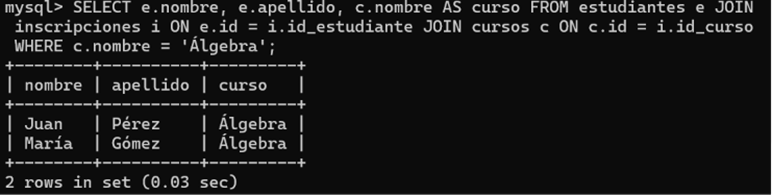
\includegraphics[width=0.75\textwidth]{imgs/pregunta1.png}
    \caption{Resultados de la pregunta 1}
\end{figure}

\begin{figure}[H]
    \centering
    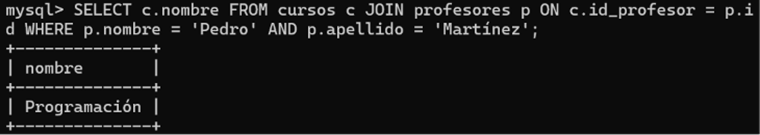
\includegraphics[width=0.75\textwidth]{imgs/pregunta2.png}
    \caption{Resultados de la pregunta 2}
\end{figure}

\begin{figure}[H]
    \centering
    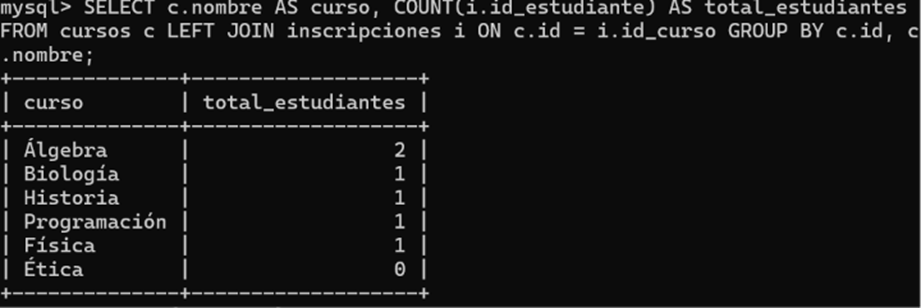
\includegraphics[width=0.75\textwidth]{imgs/pregunta3.png}
    \caption{Resultados de la pregunta 3}
\end{figure}

\begin{figure}[H]
    \centering
    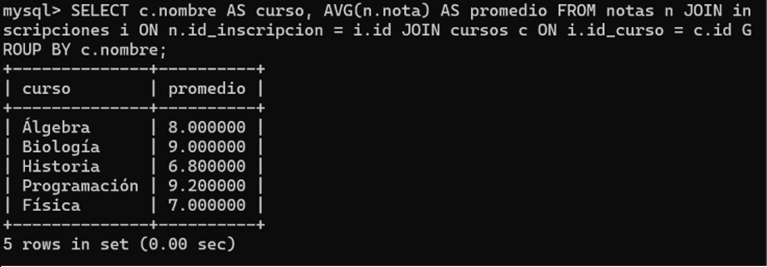
\includegraphics[width=0.75\textwidth]{imgs/pregunta4.png}
    \caption{Resultados de la pregunta 4}
\end{figure}

\begin{figure}[H]
    \centering
    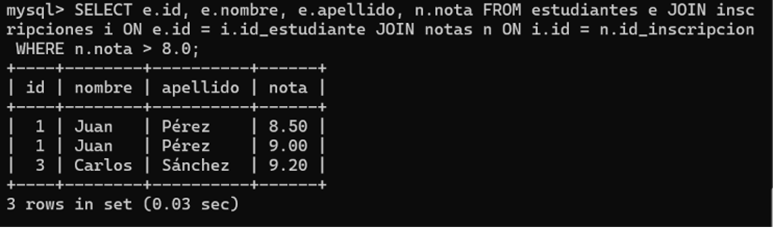
\includegraphics[width=0.75\textwidth]{imgs/pregunta5.png}
    \caption{Resultados de la pregunta 5}
\end{figure}

\begin{figure}[H]
    \centering
    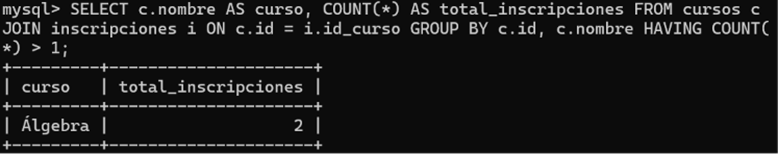
\includegraphics[width=0.75\textwidth]{imgs/pregunta6.png}
    \caption{Resultados de la pregunta 6}
\end{figure}

\begin{figure}[H]
    \centering
    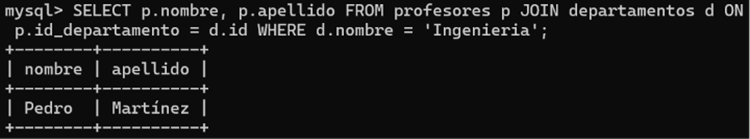
\includegraphics[width=0.75\textwidth]{imgs/pregunta7.png}
    \caption{Resultados de la pregunta 7}
\end{figure}

\begin{figure}[H]
    \centering
    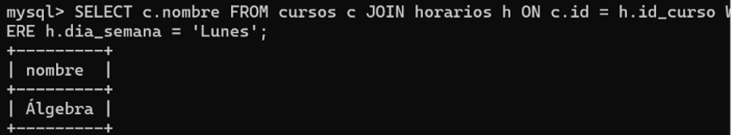
\includegraphics[width=0.75\textwidth]{imgs/pregunta8.png}
    \caption{Resultados de la pregunta 8}
\end{figure}

\begin{figure}[H]
    \centering
    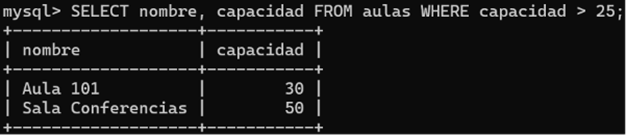
\includegraphics[width=0.75\textwidth]{imgs/pregunta9.png}
    \caption{Resultados de la pregunta 9}
\end{figure}

\begin{figure}[H]
    \centering
    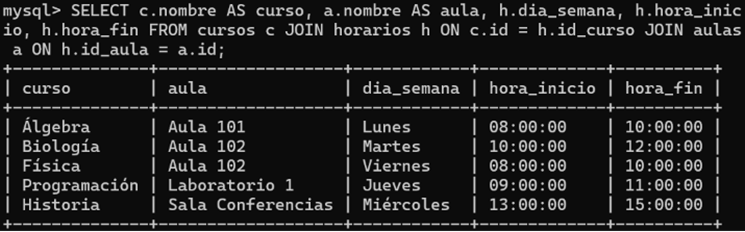
\includegraphics[width=0.75\textwidth]{imgs/pregunta10.png}
    \caption{Resultados de la pregunta 10}
\end{figure}

\begin{figure}[H]
    \centering
    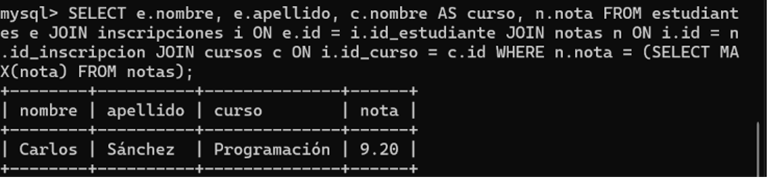
\includegraphics[width=0.75\textwidth]{imgs/pregunta11.png}
    \caption{Resultados de la pregunta 11}
\end{figure}

\begin{figure}[H]
    \centering
    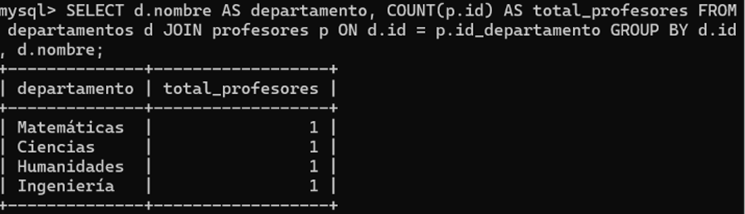
\includegraphics[width=0.75\textwidth]{imgs/pregunta12.png}
    \caption{Resultados de la pregunta 12}
\end{figure}

\begin{figure}[H]
    \centering
    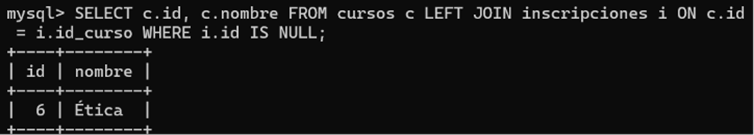
\includegraphics[width=0.75\textwidth]{imgs/pregunta13.png}
    \caption{Resultados de la pregunta 13}
\end{figure}

\begin{figure}[H]
    \centering
    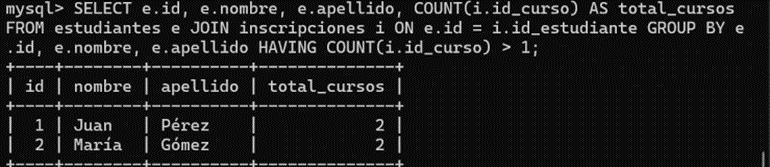
\includegraphics[width=0.75\textwidth]{imgs/pregunta14.png}
    \caption{Resultados de la pregunta 14}
\end{figure}

\begin{figure}[H]
    \centering
    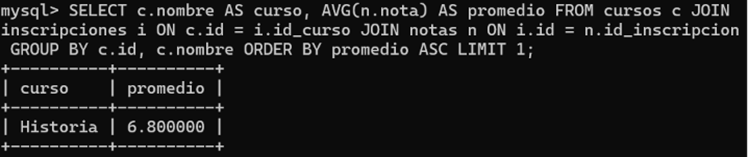
\includegraphics[width=0.75\textwidth]{imgs/pregunta15.png}
    \caption{Resultados de la pregunta 15}
\end{figure}

\section{Conclusiones}

\end{document}